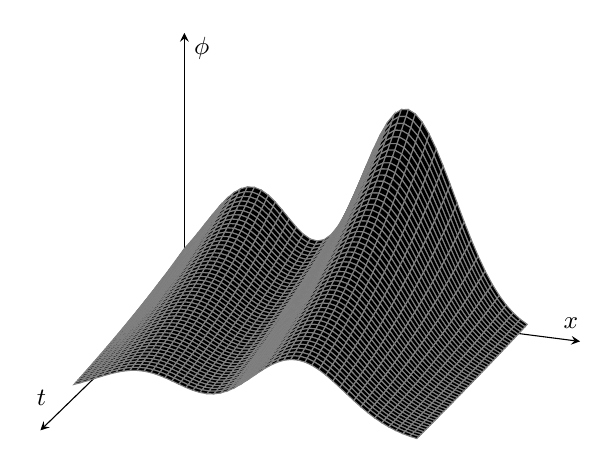
\begin{tikzpicture} [font = \small]
    \begin{axis} [
        view = {110} {30},
        xmin = 0, xmax = 3,
        ymin = 0, ymax = 7.5,
        zmin = 0, zmax = 1.1,
        axis x line = center,
        axis y line = center,
        axis z line = center,
        xtick = {0},
        xlabel = {$t$},
        ytick = {0},
        ylabel = {$x$},
        ztick = {0},
        zlabel = {$\phi$},
    ] \addplot3 [
        domain = 0:2.3,
        domain y = 0:6.5,
        samples = 50,
        samples y = 50,
        surf,
        fill = black,
        faceted color = gray,
        ] {(exp(-((y-3)/2)^2)*(1 + (0.7)*cos(70*y))*exp(-x*(0.5)))};
    \end{axis}
\end{tikzpicture}